\section{Small Training Data sets(tentative)}
\label{sec: small_data_sets}

\subsection{WHY Small Training Data Sets}
Like prior works\cite{nam2013transfer,ma2012transfer,rahman2012recalling,ryu2014value,zhang2014towards}, the basic HDP method we proposed uses all the instances in feasible data sets as training data to perform KS-test and build defect prediction learners. The straightforward drawback of using all data is that it will take much long time to finish the whole defect prediction process. The observation from our experiments also verifies this: it takes several days on a 24-cores machine to find all possible matched features in KS-test. On the other hand, whether using all the instances from the data set will be helpful and necessary to build defect learners in such transfer learning scenario is still unclear. In CPDP with transfer learning methods, where data size has a big effect on running time, small training data seems more promising if we can get similar or even better prediction performance. one of our authors, Menzies, pointed out that ``performance ceiling'' exists when using static code features to explore defects in software data repositories\cite{menzies2008implications}.  Furthermore, Thurhan et atl.\cite{turhan2009relative} and Fayola et al.\cite{peters2013better} improved the  performance of the CPDP with the same metric set by applying data filtering techniques to select the filtered training data. Therefore, it is necessary to investigate whether using small sampled data sets is feasible in heterogeneous defect prediction

\begin{figure}[!htp]
	\centering
% 	\vspace{0.5mm}
	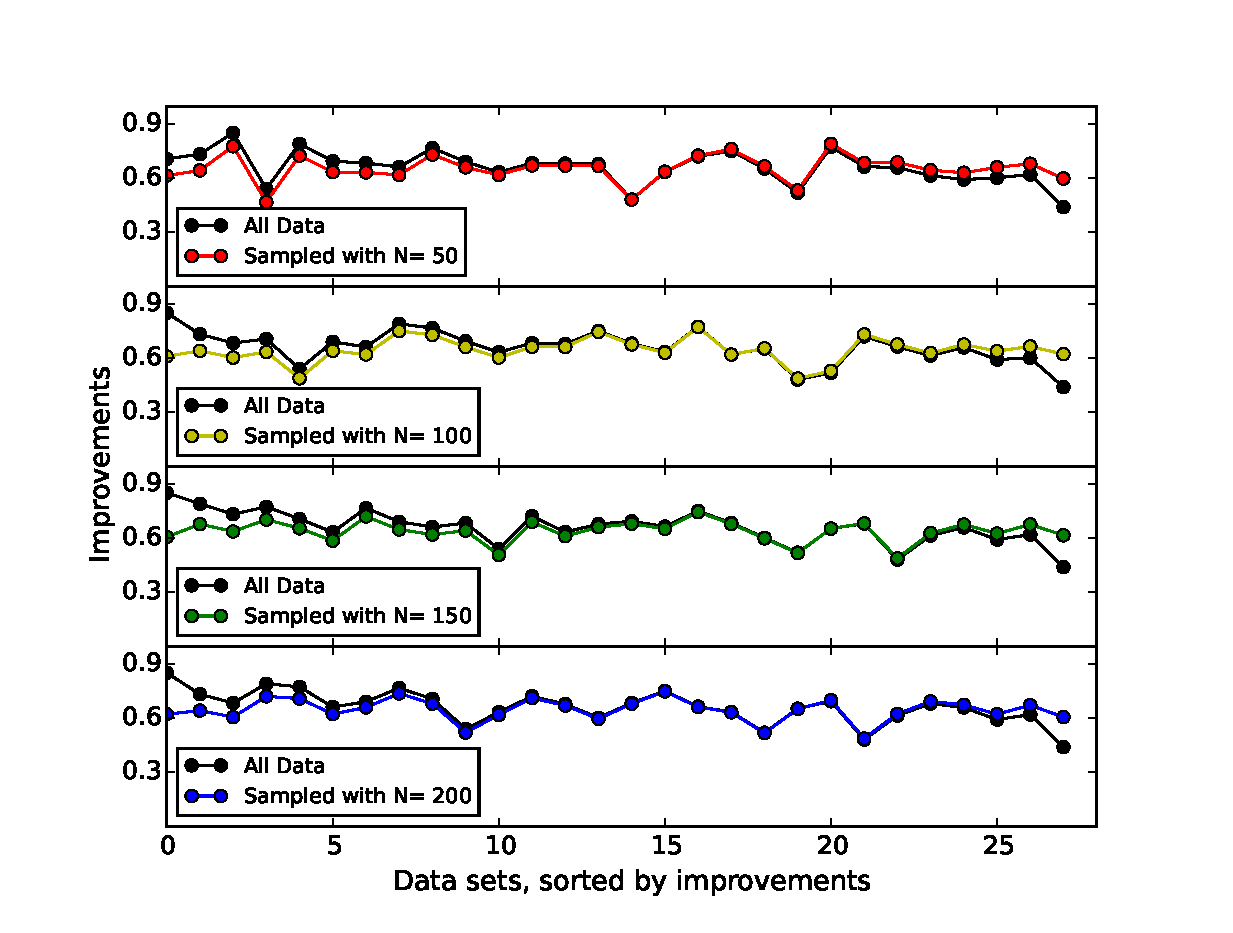
\includegraphics[width=\linewidth]{Figures/raleigh/sampled.eps}
	\caption{Improvements of using sampled data over all data with sampled size N = \{50, 100, 150, 200\}}
	\label{fig:small_data}
\end{figure}

\subsection{Approach}

In \cite{menzies2008implications}, Menzies et al. used Naive Bayes and C4.5 two simple learners to predict defects over PROMISE data. To look for the lower bound on the number of training instances, three sub-sampling techniques were applied to the training data. They found that as few as 50 instances did just as well as larger sample size and 25 might suffice for some data sets. However, in \cite{peduzzi1996simulation}, it was reported that number of events per variable(EPV) would affect the performance of logistic regression. Specifically, if the training data has fewer events relative to the independent variable, the bias of the regression coefficients will be increased.  In HDP method, data sets are used in metric selection, metric matching and learner building, where are exactly we expect to use small data size. The new experiment is designed as fowllowing.

Recall Figure \ref{fig:framework}, for the source data A, instead using all data in Project A, we perform supervised sampling with EPV =10 (recommended in \cite{peduzzi1996simulation})  and N =\{50, 100, 150, 200\} instances will be selected as the new source data ${\hat A}$, which will be used in metric selection, metric matching and prediction phases. For the target project B, instead of using all data for metric matching, a unsupervised sampling applied into project B and resultant data sets ${\hat B}$ with N = \{50, 100, 150, 200\} instances will be only used for metric matching. After prediction model is built with new source data $\hat A$, the original target data B will be applied to predict defects. Note that based on previous HDP experiments, the number of matched metrics(variables) is round 2. Therefore, at most 20 defective instances are randomly selected from source data in supervised sampling.

\subsection{Discussion}
As seen in Figure \ref{fig:small_data}, we can get the similar performance as the original experiment even with the only subset of the original data sets. As $N$ increases from 50 to 200, the performance doesn't change a lot.


